
\section{Methodology}
\label{sec:methodology}

	This section outlines our system design to overcome the facilitate distributed state synchronization. We propose a distributed server model (see Figure~\ref{figure:server-models}(b)) to enable graceful failure handling in our system. In this model, clients are paired with servers that run on the same machine. This arrangement results in a \emph{fate sharing} between client server pairs. Paired servers validate actions performed by corresponding clients. If the server finds the action valid, the action of broadcast by the server to other nodes. The following subsections will discuss each component in the proposed architecture in detail.

\begin{figure}[ht]
	\centering
	\begin{tabular}{c c}
		
		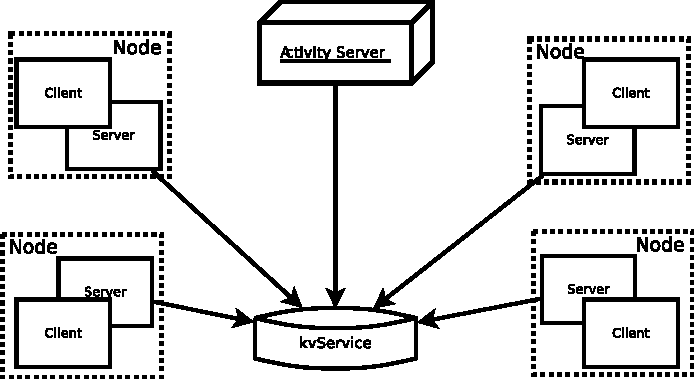
\includegraphics[width=0.52\linewidth]{../images/client-distributed-server-model-Activity-crop.pdf} &
		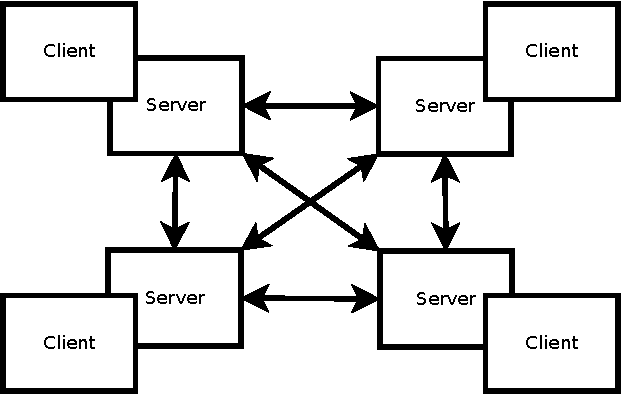
\includegraphics[width=0.40\linewidth]{../images/client-distributed-server-model-crop.pdf} \\
		(a) & (b)
	\end{tabular}
	\caption{\label{figure:server-models} Figure (a) shows servers interacting with \activityServer and \kvService. In this model all of the servers periodically update their entry in the \kvService and the \activityServer periodically publishes a list of online servers in the \kvService. The model in figure (b) shows node-node communication in general.}

\end{figure}


\subsection{The Client}

	In general, the client provides an interface to the user/player. Through this interface a player can give commands to their character (referred to as agent) in the game. The client simulates a local version of the game, where the player's commands are executed. %The commands executed by player on his agent produce changes in the state of the agent. 
	
	Each client in the system is paired with a server (called a \localServer) which acts as a proxy to all distributed servers in the system. The state of a client's agent is forwarded to the \localServer periodically. 
	
\subsection{The (Local) Server}

	The \localServer also simulates its own independent version of the game. The \gamestate at the \localServer is guided in coordination with the other nodes in the system. The purpose of the \localServer is not just to reduce message passing but also to act as a validator/authority over the client's \gamestate and actions, to prevent malicious clients from propagating invalid information. The authoritative server for a particular client depends on the event/action being processed. Any client update is first forwarded to its \localServer where it is validated against the current \gamestate of the \localServer. The update is published only if the requested action or update is found valid, else the action is rejected by the \localServer and the client's state may be overridden by the \localServer. 
	
\subsection{The Activity Server}

	The purpose of \activityServer is to support the architecture of the system, which includes allowing a new nodes to join the system and publishing the list of nodes which are currently active. The \activityServer doesn't perform game simulation, nor involves itself in game semantic actions.

\subsection{The Key-Value Service}

	The \kvService is a hash table which acts as a communication channel between different system components. The sole purpose of this service is to provide the \activityServer with a means to publish a list of active nodes. The nodes periodically update an entry in the \kvService and based on those entry updates, the \activityServer publishes a list of nodes which are currently active. This list is periodically fetched by the nodes to determine which nodes are currently active.

\subsection{ARM Game}

	This system support an Asynchronous Real-time Multiplayer Game (ARM Game). It consists of a few standard actions for players (characterized as agents in the game). The first action is a \emph{Move} which is represented as \move{\agent}{\position}, where the first argument represents the agent intended to be moved and the second argument is the agent's new location. The other action is \emph{Fire} which is represented as \fire{\position}{\direction}, where the first argument represents current position of the agent firing the shot and the second argument represents the direction in which the shot is fired.
	
	In order to simulate the game, information is needed on the other agents in the game. The information corresponding to each agent is called the \agentstate. The attributes of \agentstate are shown in Table~\ref{table:gamestate-struct}. A collective database storing \agentstate of all agents in the game is known as \gamestate.  
	
	
\subsubsection{Protocol and Messaging}

 All communication is asynchronous without acknowledgements. We use messages formatted in JSON to facilitate information exchange in the system. 


	
